\subsection{Lid-driven cavity 3d}
We consider the 3D lid-diven cavity problem to verify our code Navier-Stokes in 3D. The flow is confined in a cube which is given from extending the 2D domain in the z-direction with the width $1$. We impose the Dirichlet boundary conditions: $u_x = 1, u_y = 0, u_z = 0 $ in the plane $y=1$ and initial zero-velocity for other planes. Two mesh employed to simulate 3D problem: the coarse one consists of 11037 vertices, 56244 tetrahedrals for the cases of $Re = 100, \, Re = 400$ and the other one consists of 35723 vertices, 193586 tetrahedrals for $Re = 1000$. 
In many references the results in 3D is examined by plane in 2D, so we simulate 3D problem with the same number of Reynolds in 2D: $Re = 100,\, Re = 400, \,Re =1000$.
As expected, we obtain the streamlines in the each plane $z=const$ are correspondent to those in 2D, see the figure \ref{streamline3D} for example.
\begin{figure}[htbp]
\begin{minipage}[b]{0.5\textwidth}
\centering
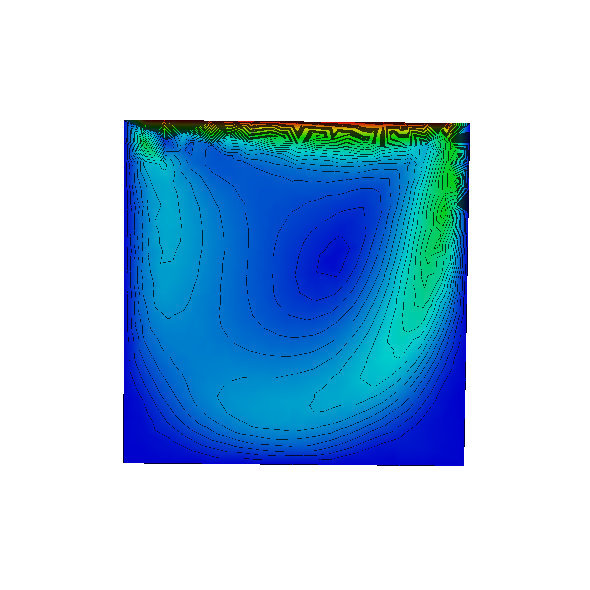
\includegraphics[height=9cm,width=9cm]{cavity3d/cube1_400}
\end{minipage}
\hfill
\begin{minipage}[b]{0.5\textwidth}
\centering
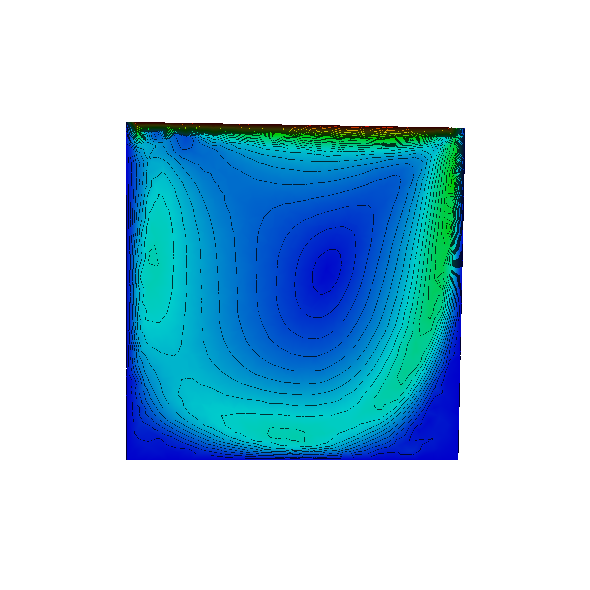
\includegraphics[height=9cm,width=9cm]{cavity3d/cube2_1000}
\end{minipage}
\caption{\em Cavity in 3D: streamlines in the plane ($z=0.5$) for Re = 400 (left), Re = 1000 (right)}\label{streamline3D}
\end{figure}\\
We would like to compare our numerical solutions with the results in \cite{Ku87} because the numbers of Reynolds are exactly the same in our tests, but we didn't see the details of data of velocity profiles, so we show the images of our velocity profiles in 2D, 3D and those obtained in given reference. The comparison is in good agreements showed in the Figure \ref{Ku}
%\ref{Ku100x}, \ref{Ku100y}, \ref{Ku400x}, \ref{Ku400y}, \ref{Ku1000x}, \ref{Ku1000y}.
\newpage
\begin{figure}[htbp]
\centering
\begin{tabular}{c}
\hspace{-0.5cm} 
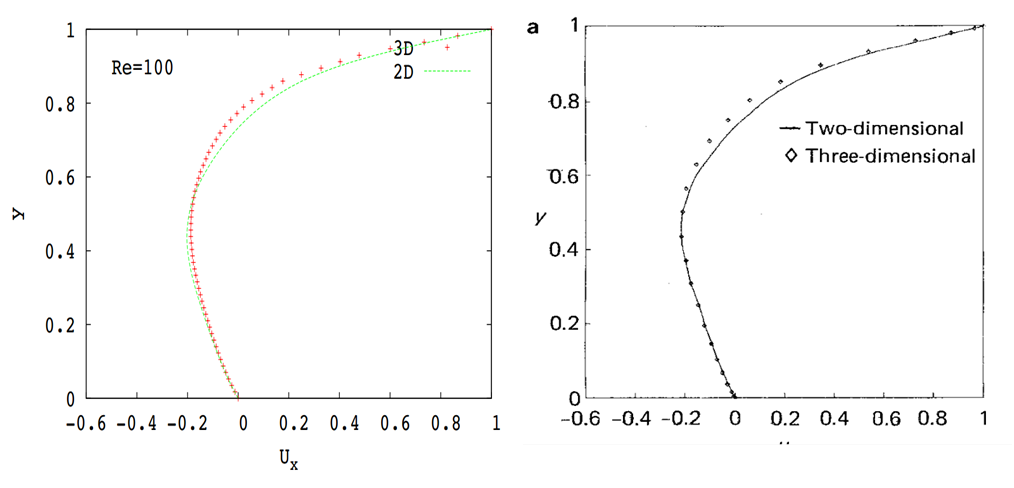
\includegraphics[height=4cm,width=10cm]{cavity3d/100x}\\
\hspace{-0.5cm} 
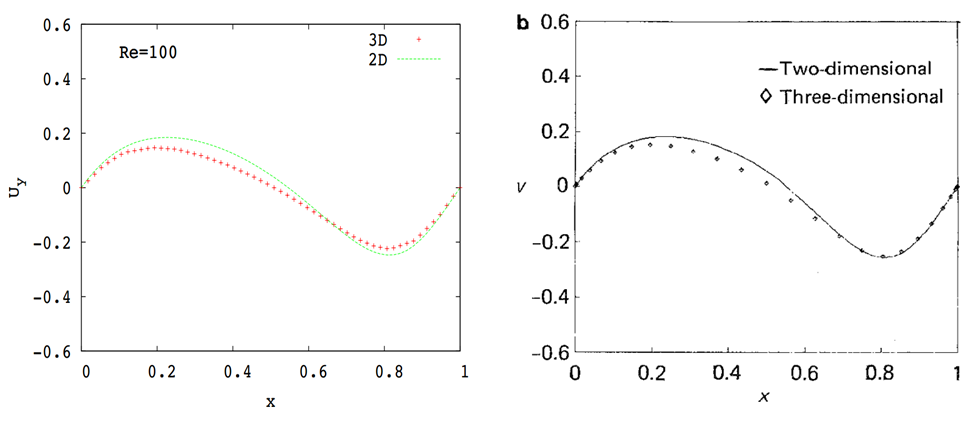
\includegraphics[height=4cm,width=10cm]{cavity3d/100y}\\
\hspace{-0.5cm} 
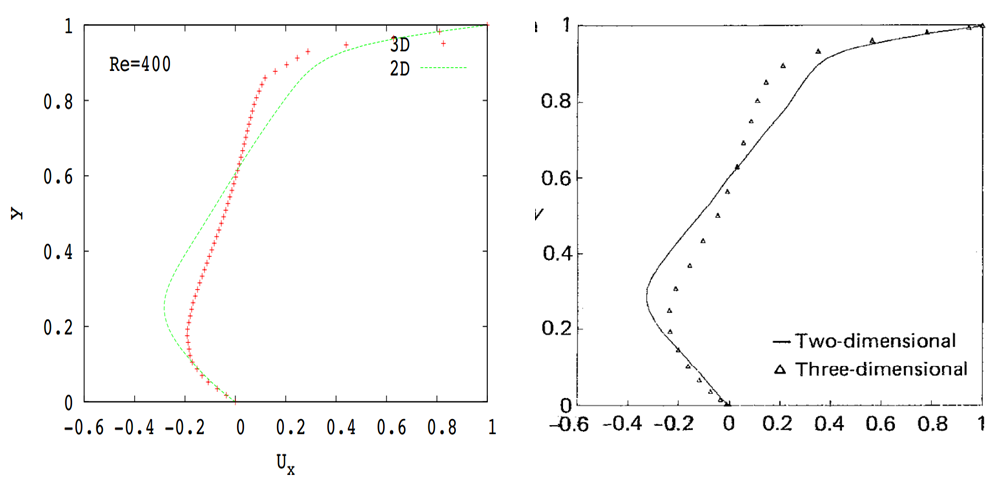
\includegraphics[height=4cm,width=10cm]{cavity3d/400x}\\
\hspace{-0.5cm} 
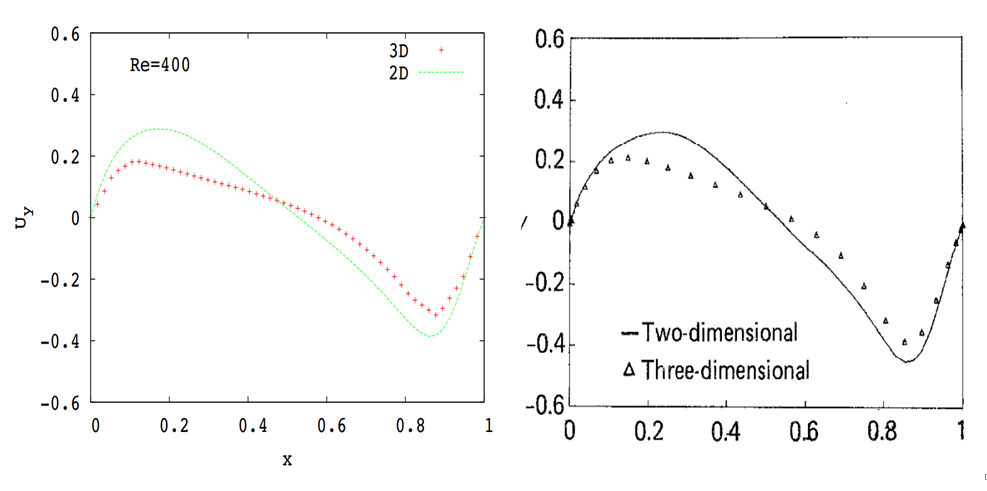
\includegraphics[height=4cm,width=10cm]{cavity3d/400y}\\
\hspace{-0.5cm}
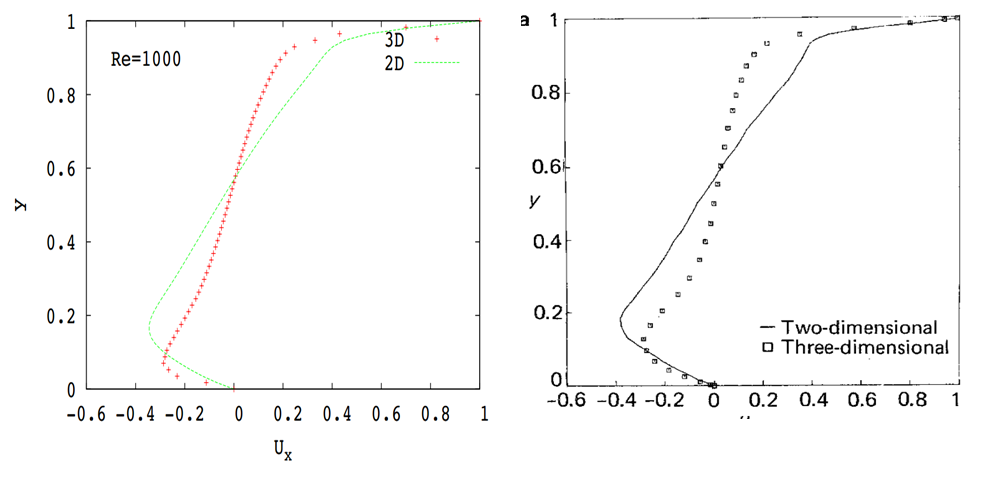
\includegraphics[height=4cm,width=10cm]{cavity3d/1000x}\\
\hspace{-0.5cm} 
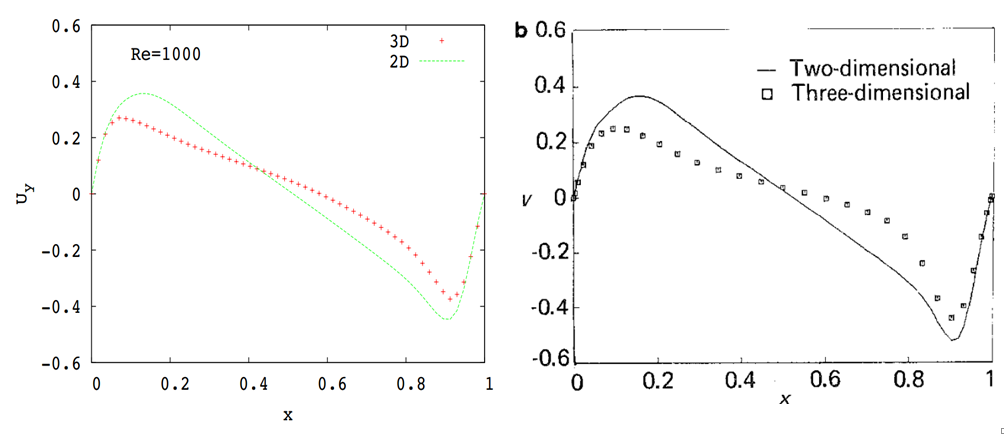
\includegraphics[height=4cm,width=10cm]{cavity3d/1000y}\\
\end{tabular}
\caption{\em Cavity in 3D: velocity profiles on vertical centerline. Left: present results. Right: results obtained in \cite{Ku87}} \label{Ku}
\end{figure}
%\begin{figure}[htbp]
%\centering
%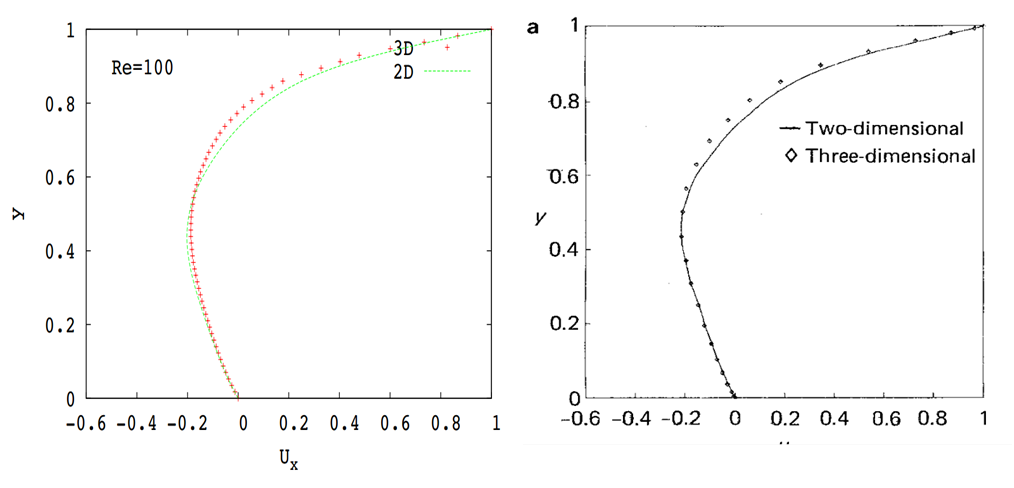
\includegraphics[height=7cm,width=15cm]{cavity3d/100x}
%\caption{Velocity profiles on vertical centerline for Re = 100. Left: present results. Right: results obtained in \cite{Ku87}} \label{Ku100x}
%\end{figure}
%\begin{figure}[htbp]
%\centering
%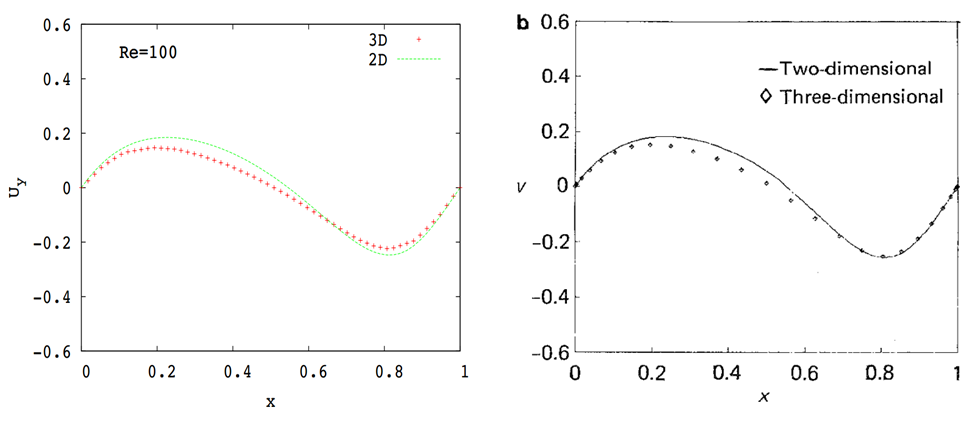
\includegraphics[height=7cm,width=15cm]{cavity3d/100y}
%\caption{Velocity profiles horizontal centerline for Re = 100. Left: present results. Right: results obtained in \cite{Ku87}}\label{Ku100y}
%\end{figure}
%\begin{figure}[htbp]
%\centering
%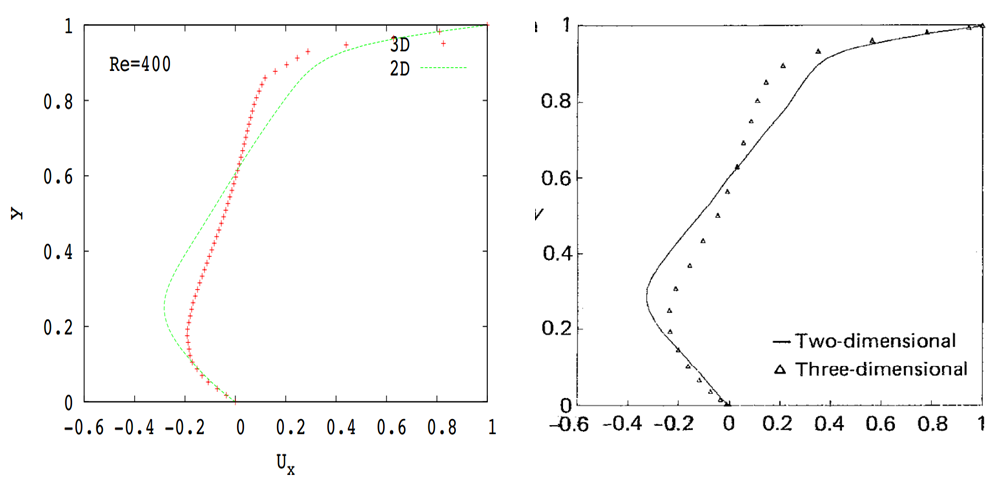
\includegraphics[height=7cm,width=15cm]{cavity3d/400x}
%\caption{Velocity profiles on vertical centerline for Re = 400. Left: present results. Right: results obtained in \cite{Ku87}}\label{Ku400x}
%\end{figure}
%\begin{figure}[htbp]
%\centering
%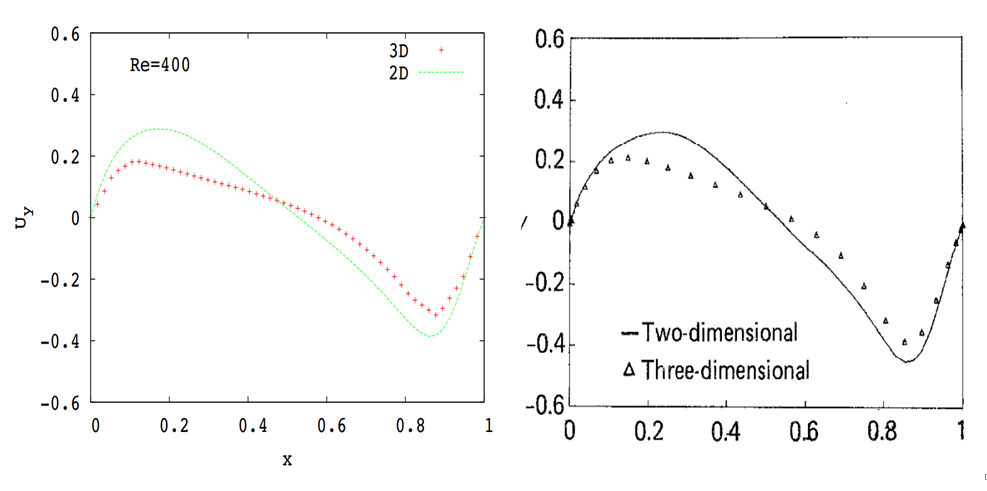
\includegraphics[height=7cm,width=15cm]{cavity3d/400y}
%\caption{Velocity profiles horizontal centerline for Re = 400. Left: present results. Right: results obtained in \cite{Ku87}}\label{Ku400y}
%\end{figure}
%\begin{figure}[htbp]
%\centering
%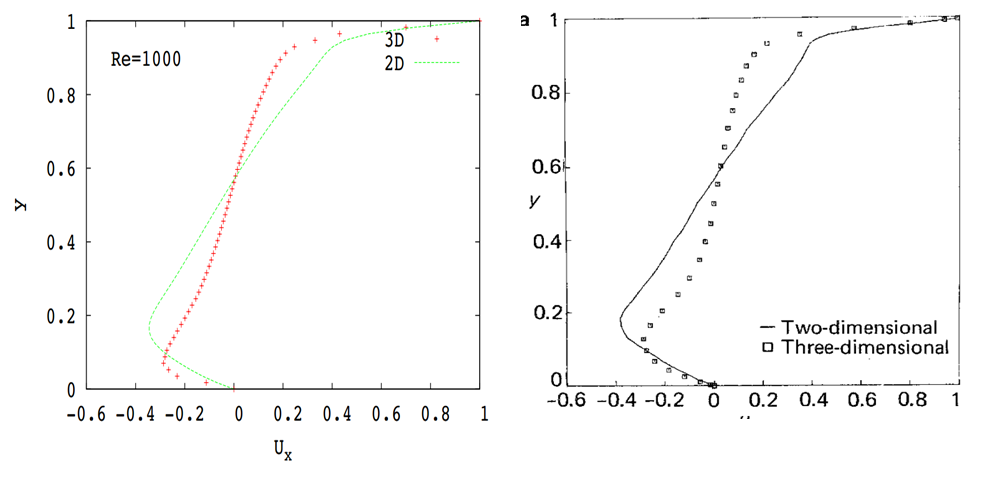
\includegraphics[height=7cm,width=15cm]{cavity3d/1000x}
%\caption{Velocity profiles on vertical centerline for Re = 1000. Left: present results. Right: results obtained in \cite{Ku87}}\label{Ku1000x}
%\end{figure}
%\begin{figure}[htbp]
%\centering
%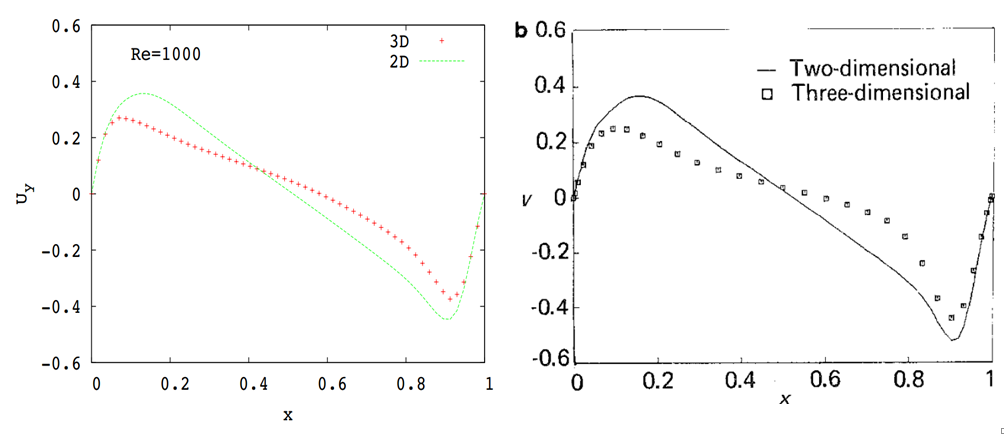
\includegraphics[height=7cm,width=15cm]{cavity3d/1000y}
%\caption{Velocity profiles horizontal centerline for Re = 100. Left: present results. Right: results obtained in \cite{Ku87}}\label{Ku1000y}
%\end{figure}\\
Our computations in 3D is also compared with the results obtained in \cite{Hac10}, the results in this reference was in perfect agreement with those of \cite{Tang95} et \cite{Yang98}, in figure \ref{Ha} we see again the satisfactory comparison with these references.
\begin{figure}[htbp]
\begin{minipage}[b]{0.5\textwidth}
\centering
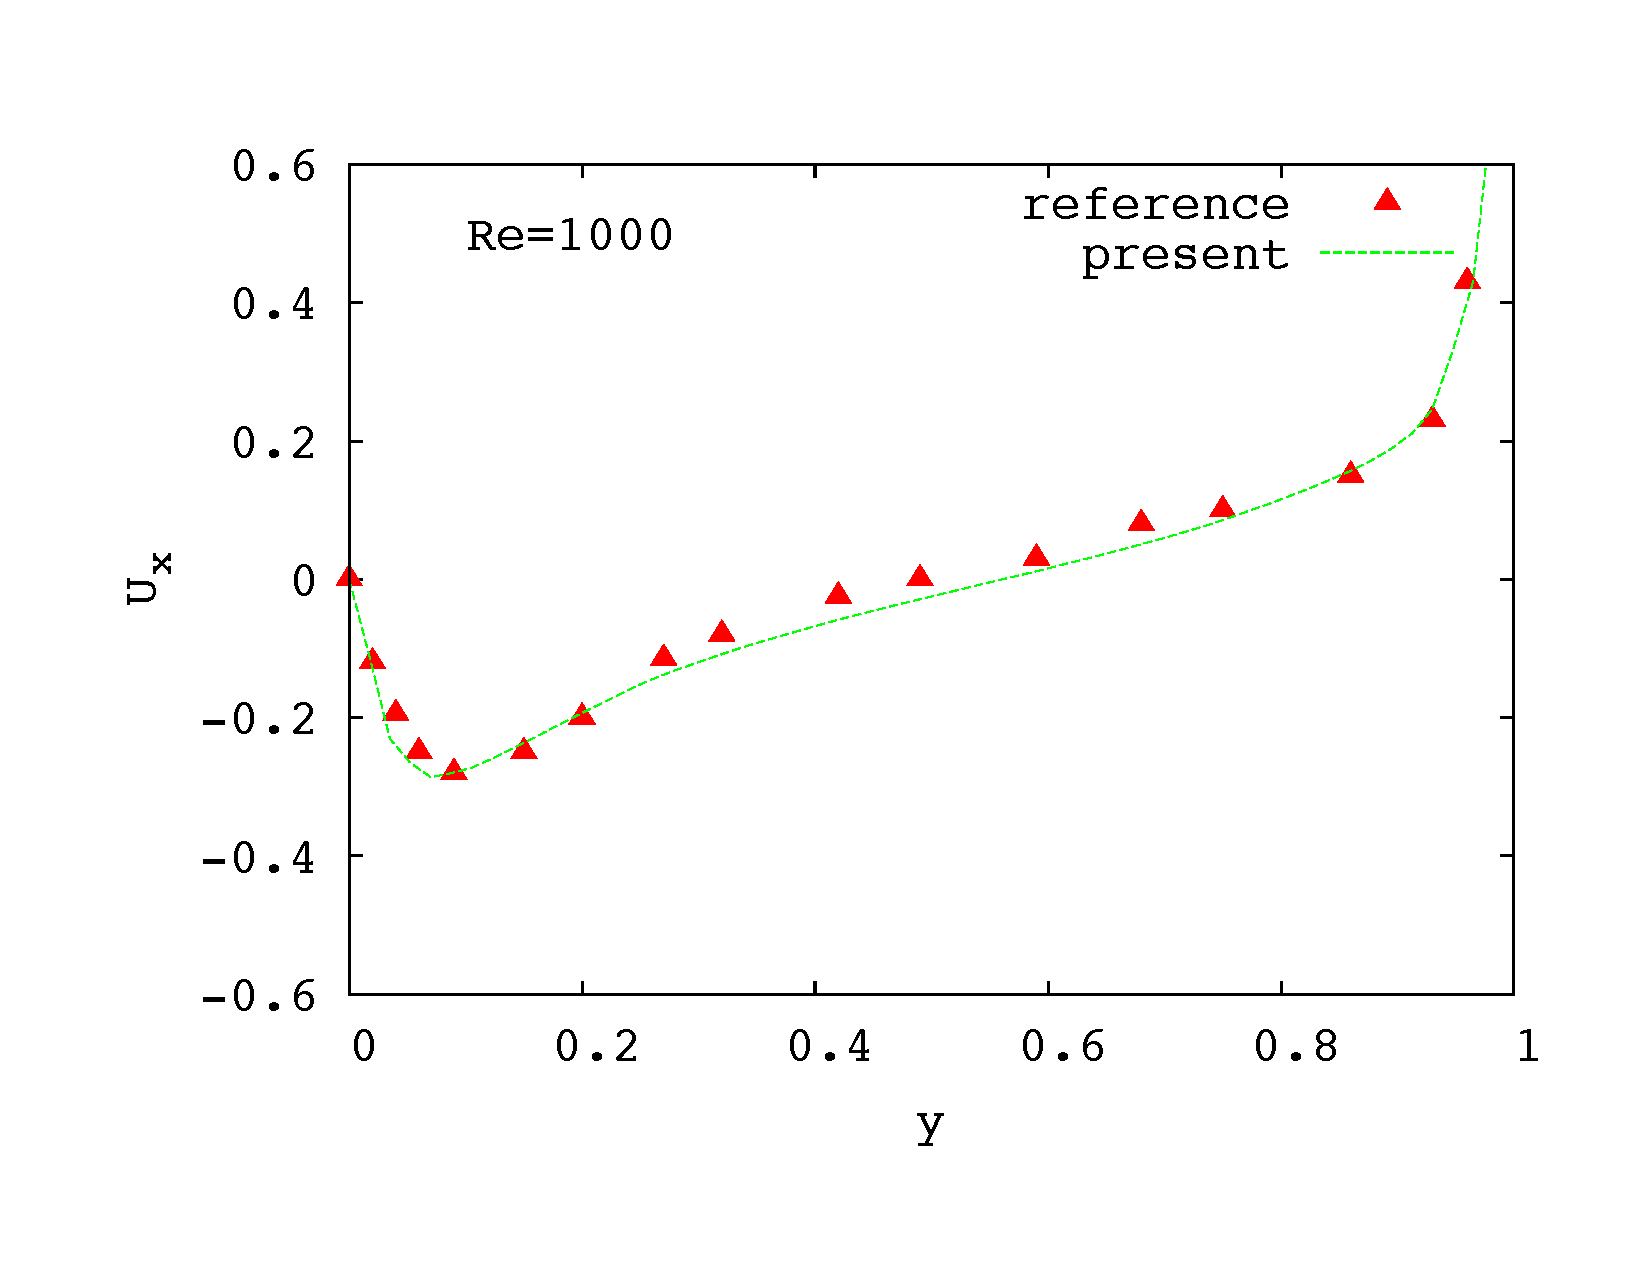
\includegraphics[height=7cm,width=8cm]{cavity3d/xHa_1000}
\end{minipage}
\hfill
\begin{minipage}[b]{0.5\textwidth}
\centering
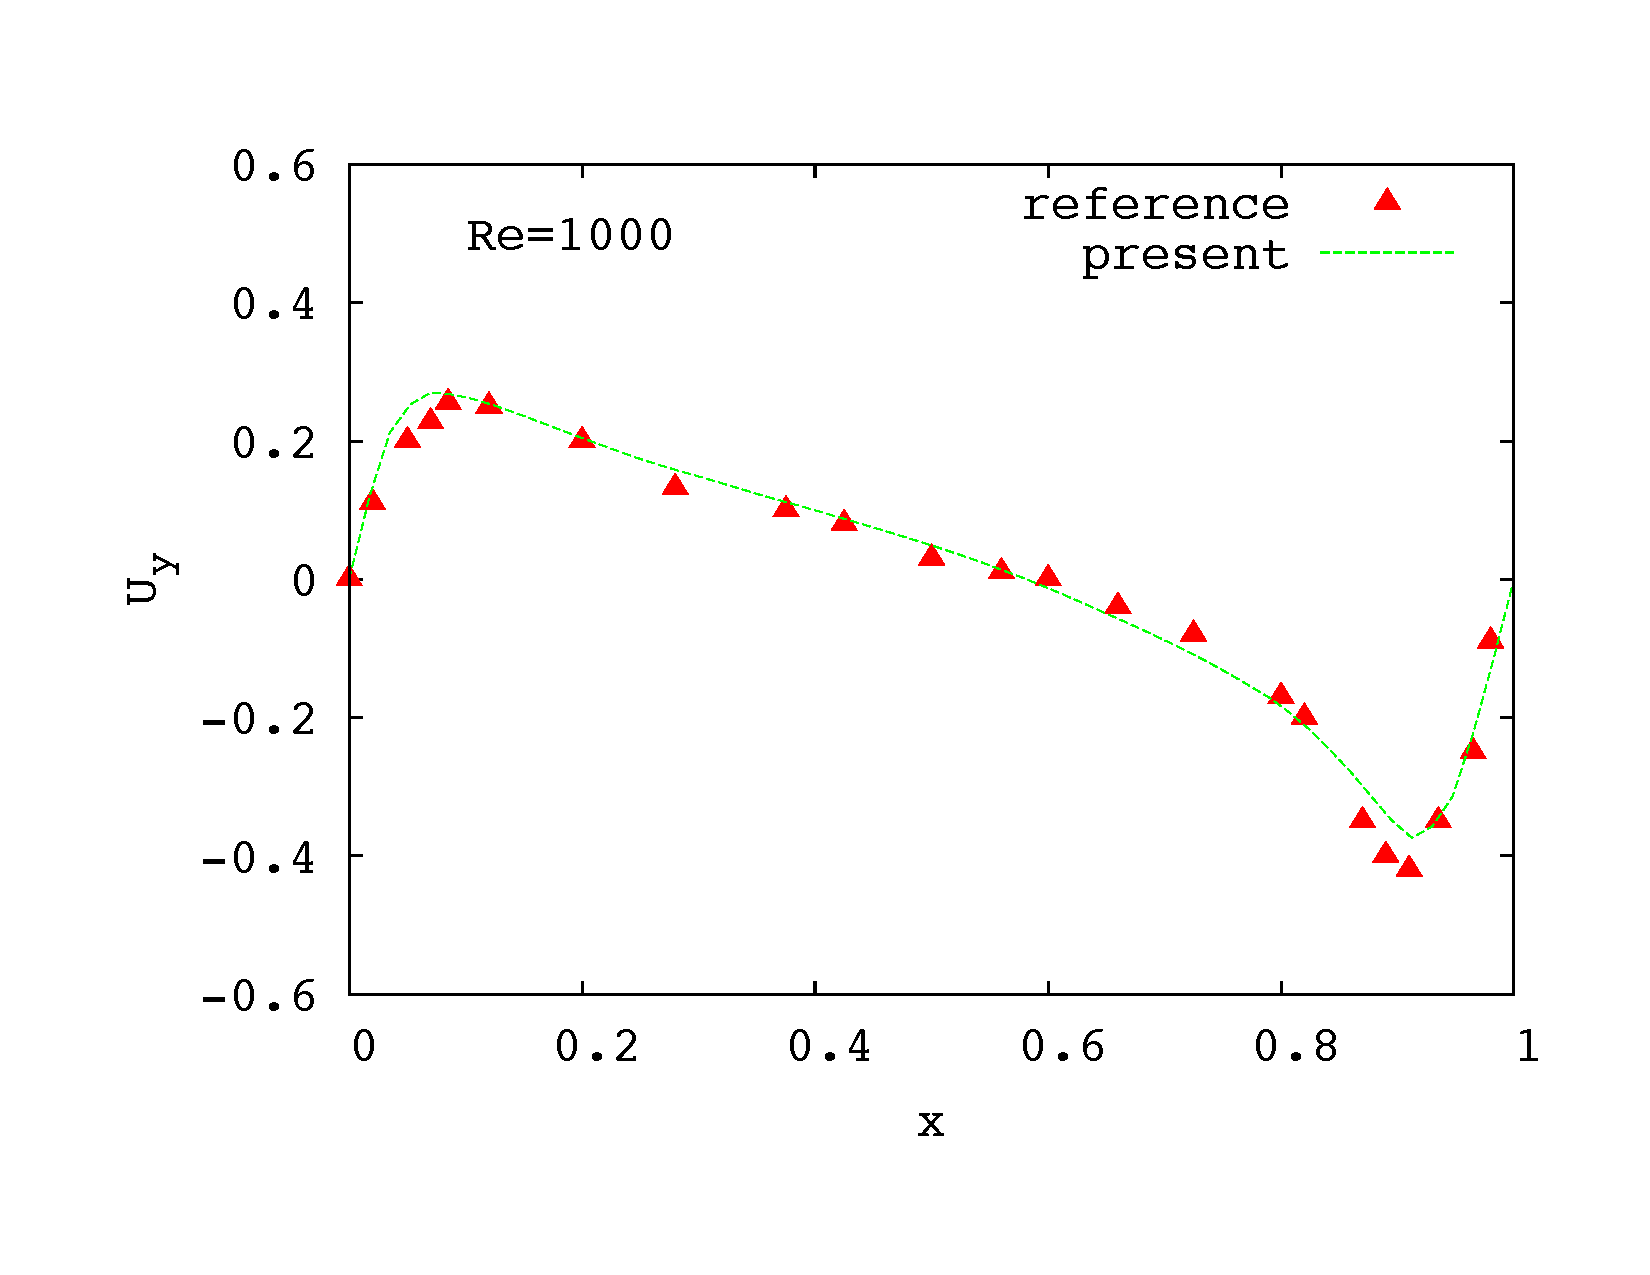
\includegraphics[height=7cm,width=8cm]{cavity3d/yHa_1000}
\end{minipage}
\caption{\em Cavity in 3D: comparison the velocity profiles $u_y$ on the vertical centerline and $u_x$ on the horizontal centerline of the symmetry plane ($z=0.5$).}\label{Ha}
\end{figure}
